
% En este capítulo explicamos como el anti-thickness puede ser explicado desde
% la definición de un concepto ampliamente estudiado, hablaremos de cómo el número
% cromático de una gráfica abstracta  está directamente relacionado con el anti-thickness también presentamos los
% resultados del anti-thickness geométrico para el caso específico de puntos
% en posición convexa.

En este capítulo hablaremos de un concepto que históricamente fue definido antes
del anti-thickness y de cómo se relacionan. Mencionamos algunos resultados acerca
de dicho concepto. Explicaremos de qué manera el número cromático de una
gráfica puede otorgar una descomposición de una gráfica geométrica basándonos
en trabajos en los que se busca obtener una descomposición de una gráfica geométrica.

Un concepto que está estrechamente relacionado con el de anti-thickness es el
de thickness que esta definido como sigue:
\begin{definition}{\emph{Thickness}.}
  El thickness de una gráfica $G$, denotado como $\theta(G)$, es la mínima $k$ tal que existe
  una partición de las aristas de $G$, cuyo tamaño es $k$ y cada elemento
  induce una gráfica planar.
\end{definition}
Este concepto también puede ser aplicado a gráficas que están encajadas en el plano,
en cuyo caso estaremos hablando del thickess geométrico, definido a continuación:
\begin{definition}{\emph{Thickness geométrico}.}
  El thickness geométrico de una gráfica $G$, denotado como $\bar{\theta}(G)$,
  es la mínima $k$ tal que existe un dibujo geométrico $\mathsf{G}$ de $G$
  el cuál tiene una partición de sus aristas, cuyo tamaño es $k$ y cada
  elemento es una gráfica plana.
\end{definition}

A través de este capítulo nos referimos a la gráfica completa de $n$ vértices
como $K_n$ ya que los trabajos citados utilizan gráficas completas y además
es también nuestro objeto de estudio.
% Antes de hablar del anti-thickness y los resultados, es sensato hablar de otro
% concepto llamado \textbf{thickness} pues su definición está estrechamente
% relacionada con el anti-thickness. En el artículo de Eppstein y otros
% \cite{Dillencourt2004} se recupera la definición de thickness teórico y thickness
% geométrico, además proporciona cotas para éste último. Podemos definir el
% thickness de una gráfica en términos del índice cromático de una gráfica y
% mantenerlo coherente con la definición de Eppstein: $\theta(G):$ Mínimo $k$
% tal que existe una partición de las aristas de $G$, de tamaño $k$ en gráficas planares.

% Por otro lado el thickness geométrico $\bar{\theta}(G)$: Mínimo $k$ tal que
% existe un dibujo geométrico $\mathsf{G}$ de $G$ cuyas aristas pueden ser
% particionadas en $k$ gráficas planas.
Respecto a este parámetro \cite{Dillencourt2004} demuestran que el thickness
geométrico está acotado por:
\[ \Bigl\lceil n/5.646 + 0.342 \Bigr\rceil \leq  \bar{\theta}(G) \leq \Bigl\lceil\frac{n}{4}\Bigr\rceil \]

En el mismo artículo encuentran el valor exacto del thicknes geométrico
de $K_n$ con $n\leq 12$ así como para $K_{15}$ y $K_{16}$. También
estudian el thickness geométrico para gráficas completas bipartitas $K_{a,b}$ y demuestran la
siguiente cota:
\[
  \Bigl\lceil \frac{ab}{2a+2b-4} \Bigr\rceil \leq \theta(K_{a,b}) \leq \bar{\theta}(K_{a,b})
  \leq \Bigl\lceil \frac{min(a,b)}{2} \Bigr\rceil
\]

A continuación citaremos dos trabajos asociados al anti-thickness cuyo núcleo
se basa en obtener el número cromático de una gráfica cuyos vértices y aristas
son abstraidas de una gráfica geométrica definida sobre un conjunto de puntos
en el plano. Empezaremos por definir la gráfica de cruce $E_{pp}(S)$ de un conjunto
de puntos $S$ en posición general. Consideremos que existe un dibujo geométrico
de $K_n$ cuyo conjunto de vértices es $S$.
\begin{definition}{\emph{Gráfica de cruce}.}
  La gráfica de cruce $E_{pp}(S)$ de un conjunto de puntos $S$ en el plano, es
  la gráfica cuyo conjunto de vértices está compuesto por todos los pares de puntos
  de $S$. Existe una arista entre dos vértices de $E_{pp}(S)$ si las aristas correspondientes
  se cruzan propiamente en $K_n$.
\end{definition}

\begin{figure}
\begin{subfigure}{.5\textwidth}
  \centering
  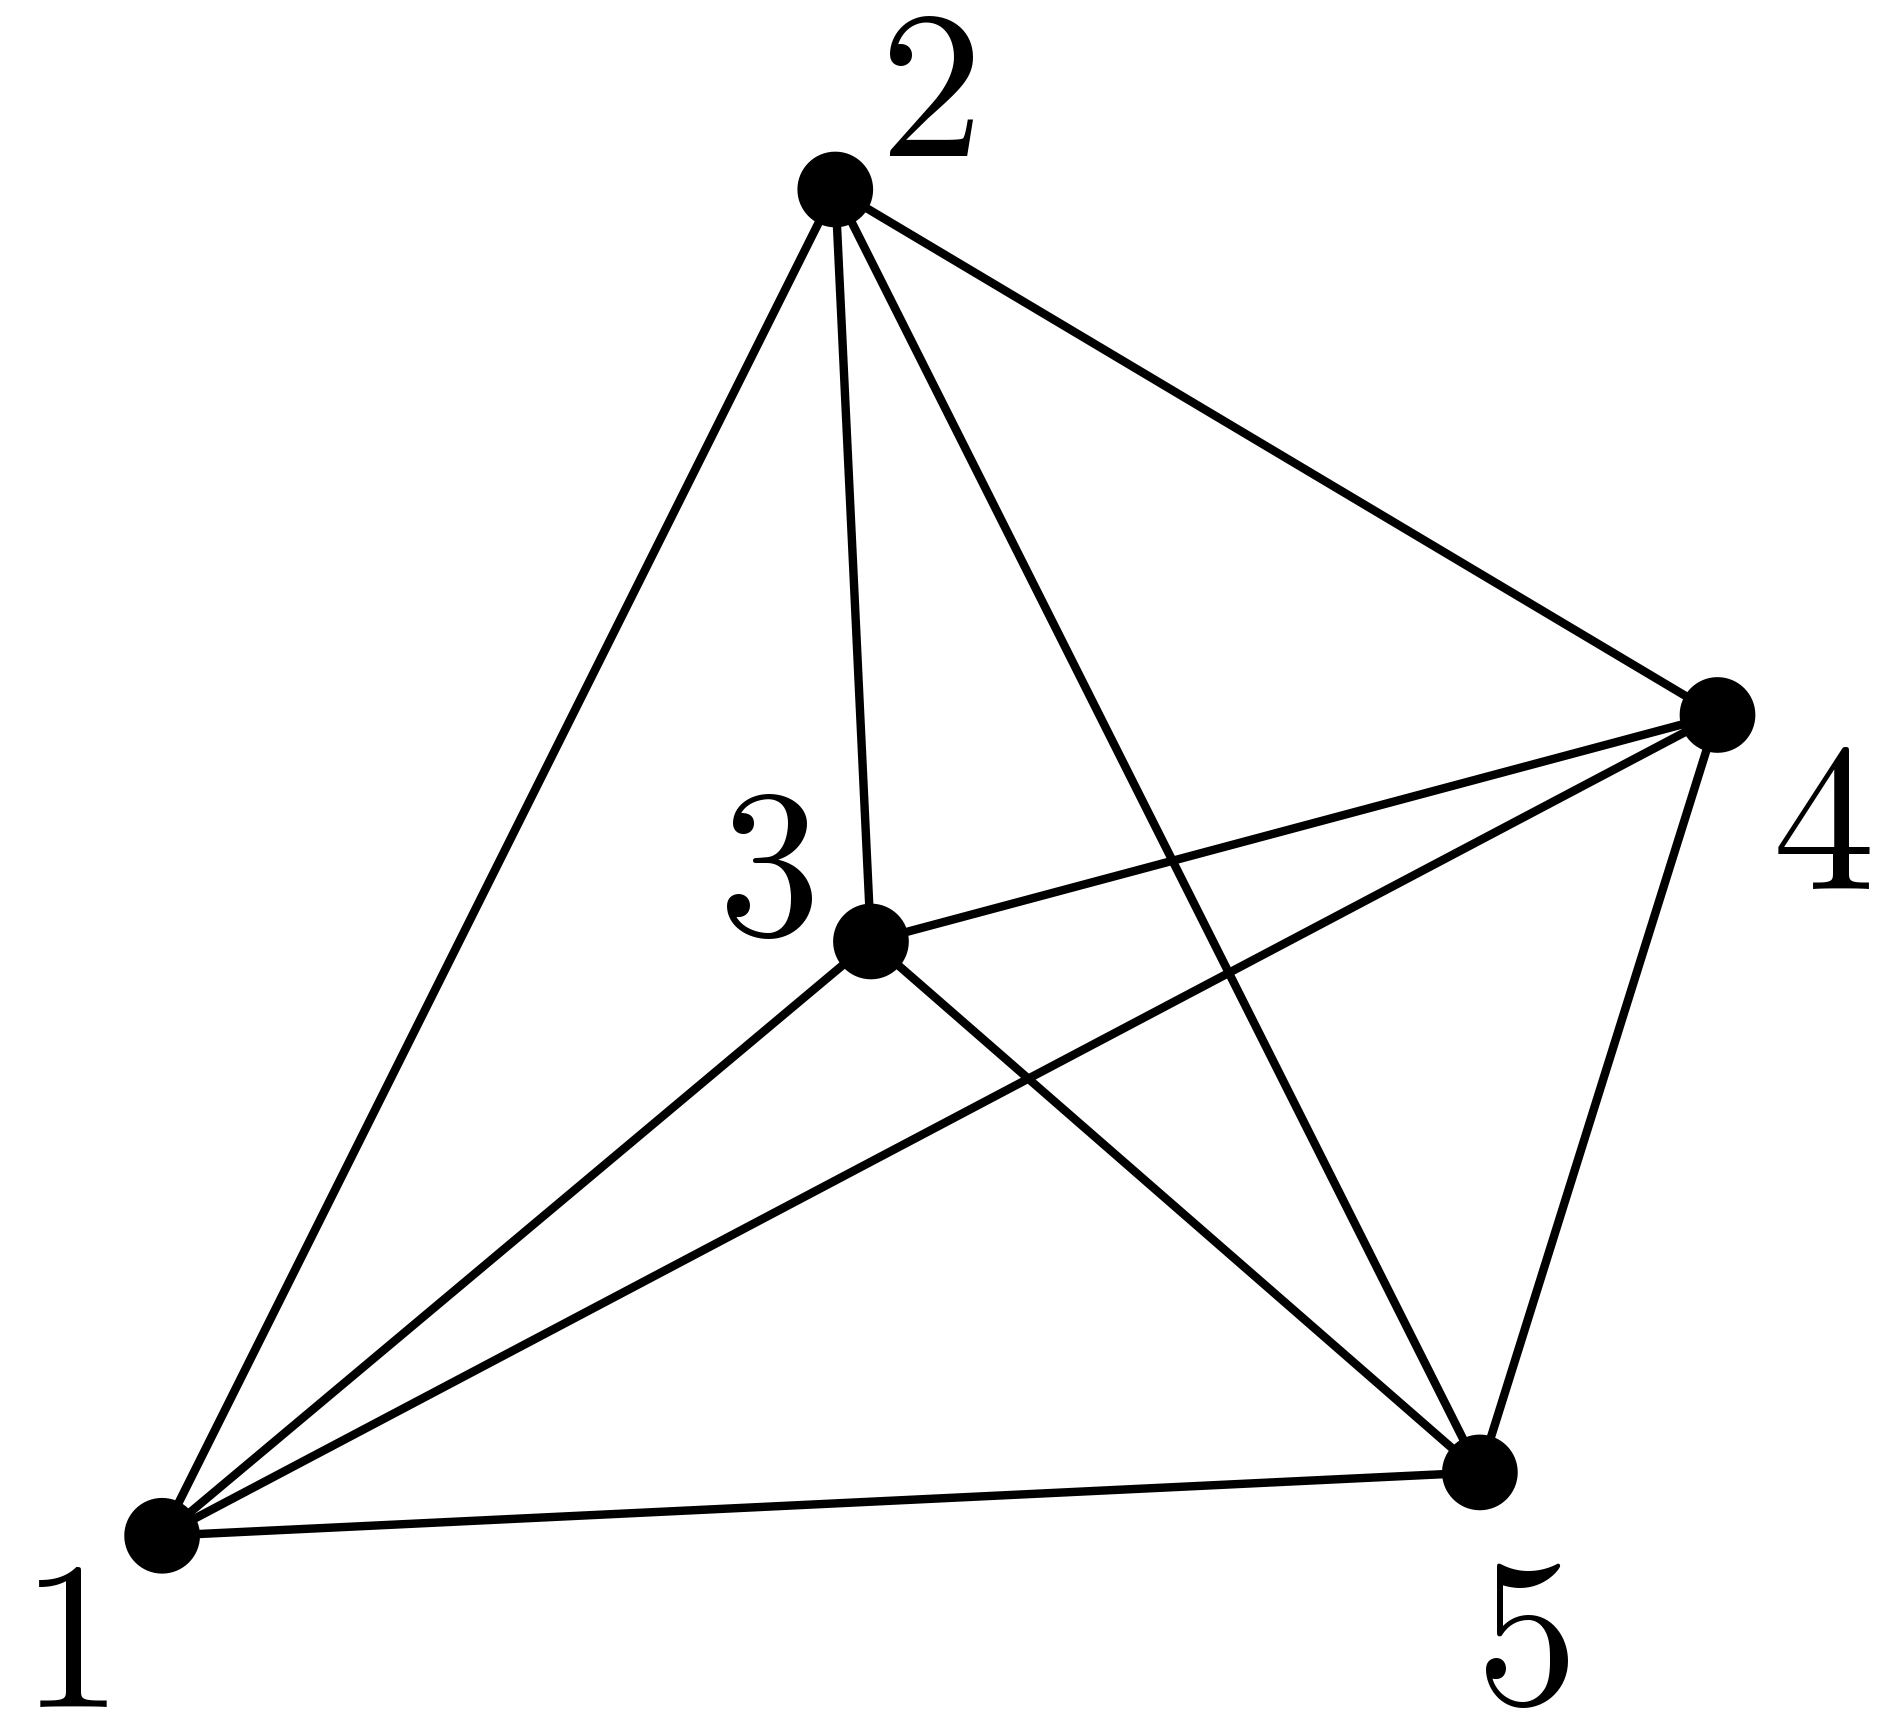
\includegraphics[width=.8\linewidth]{K5}
  \caption{Un dibujo geométrico de $K_5$ cuyo conjunto de vértices es $S=\{1,2,3,4,5\}$.}
  \label{fig:k5}
\end{subfigure}%
\begin{subfigure}{.5\textwidth}
  \centering
  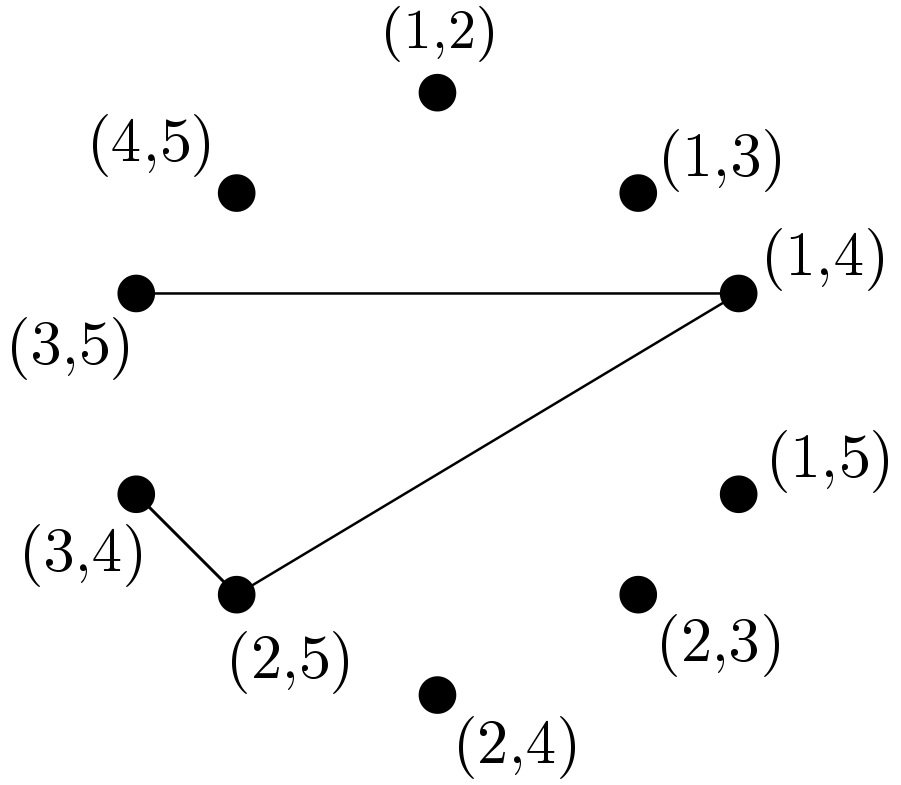
\includegraphics[width=.8\linewidth]{EppK5}
  \caption{La gráfica $E_{pp}(S)$.}
  \label{fig:eppk5}
\end{subfigure}
\caption{Una instancia de $K_5$ y su respectiva gráfica de cruce $E_{pp}(S)$.}
\label{fig:ejemploeppk5}
\end{figure}

En la figura \ref{fig:ejemploeppk5} observamos un ejemplo de la gráfica de cruce $E_{pp}(S)$.
Podemos notar que dado que en el dibujo de $K_5$ existen 3 cruces, la gráfica $E_{pp}(S)$
tiene 3 aristas.

Si analizamos ahora los conjuntos independientes de $E_{pp}(S)$ podemos verificar
que las aristas correspondientes en el dibujo de $K_n$ son en efecto gráficas planas.
Si ahora asignamos un color a cada conjunto independiente, tenemos ahora una clase
cromática por cada conjunto independiente y si minimizamos el número de clases cromáticas
habremos encontrado una coloración propia de $E_{pp}(S)$ y por consiguiente una descomposición
en gráficas planas de un dibujo de $K_n$ cuyo tamaño es mínimo, en otras palabras obtenemos
el thickness de un dibujo en particular de $K_n$. La figura \ref{fig:k5coloring}
ilustra este concepto con un dibujo de $K_5$.

\begin{figure}
  \centering
  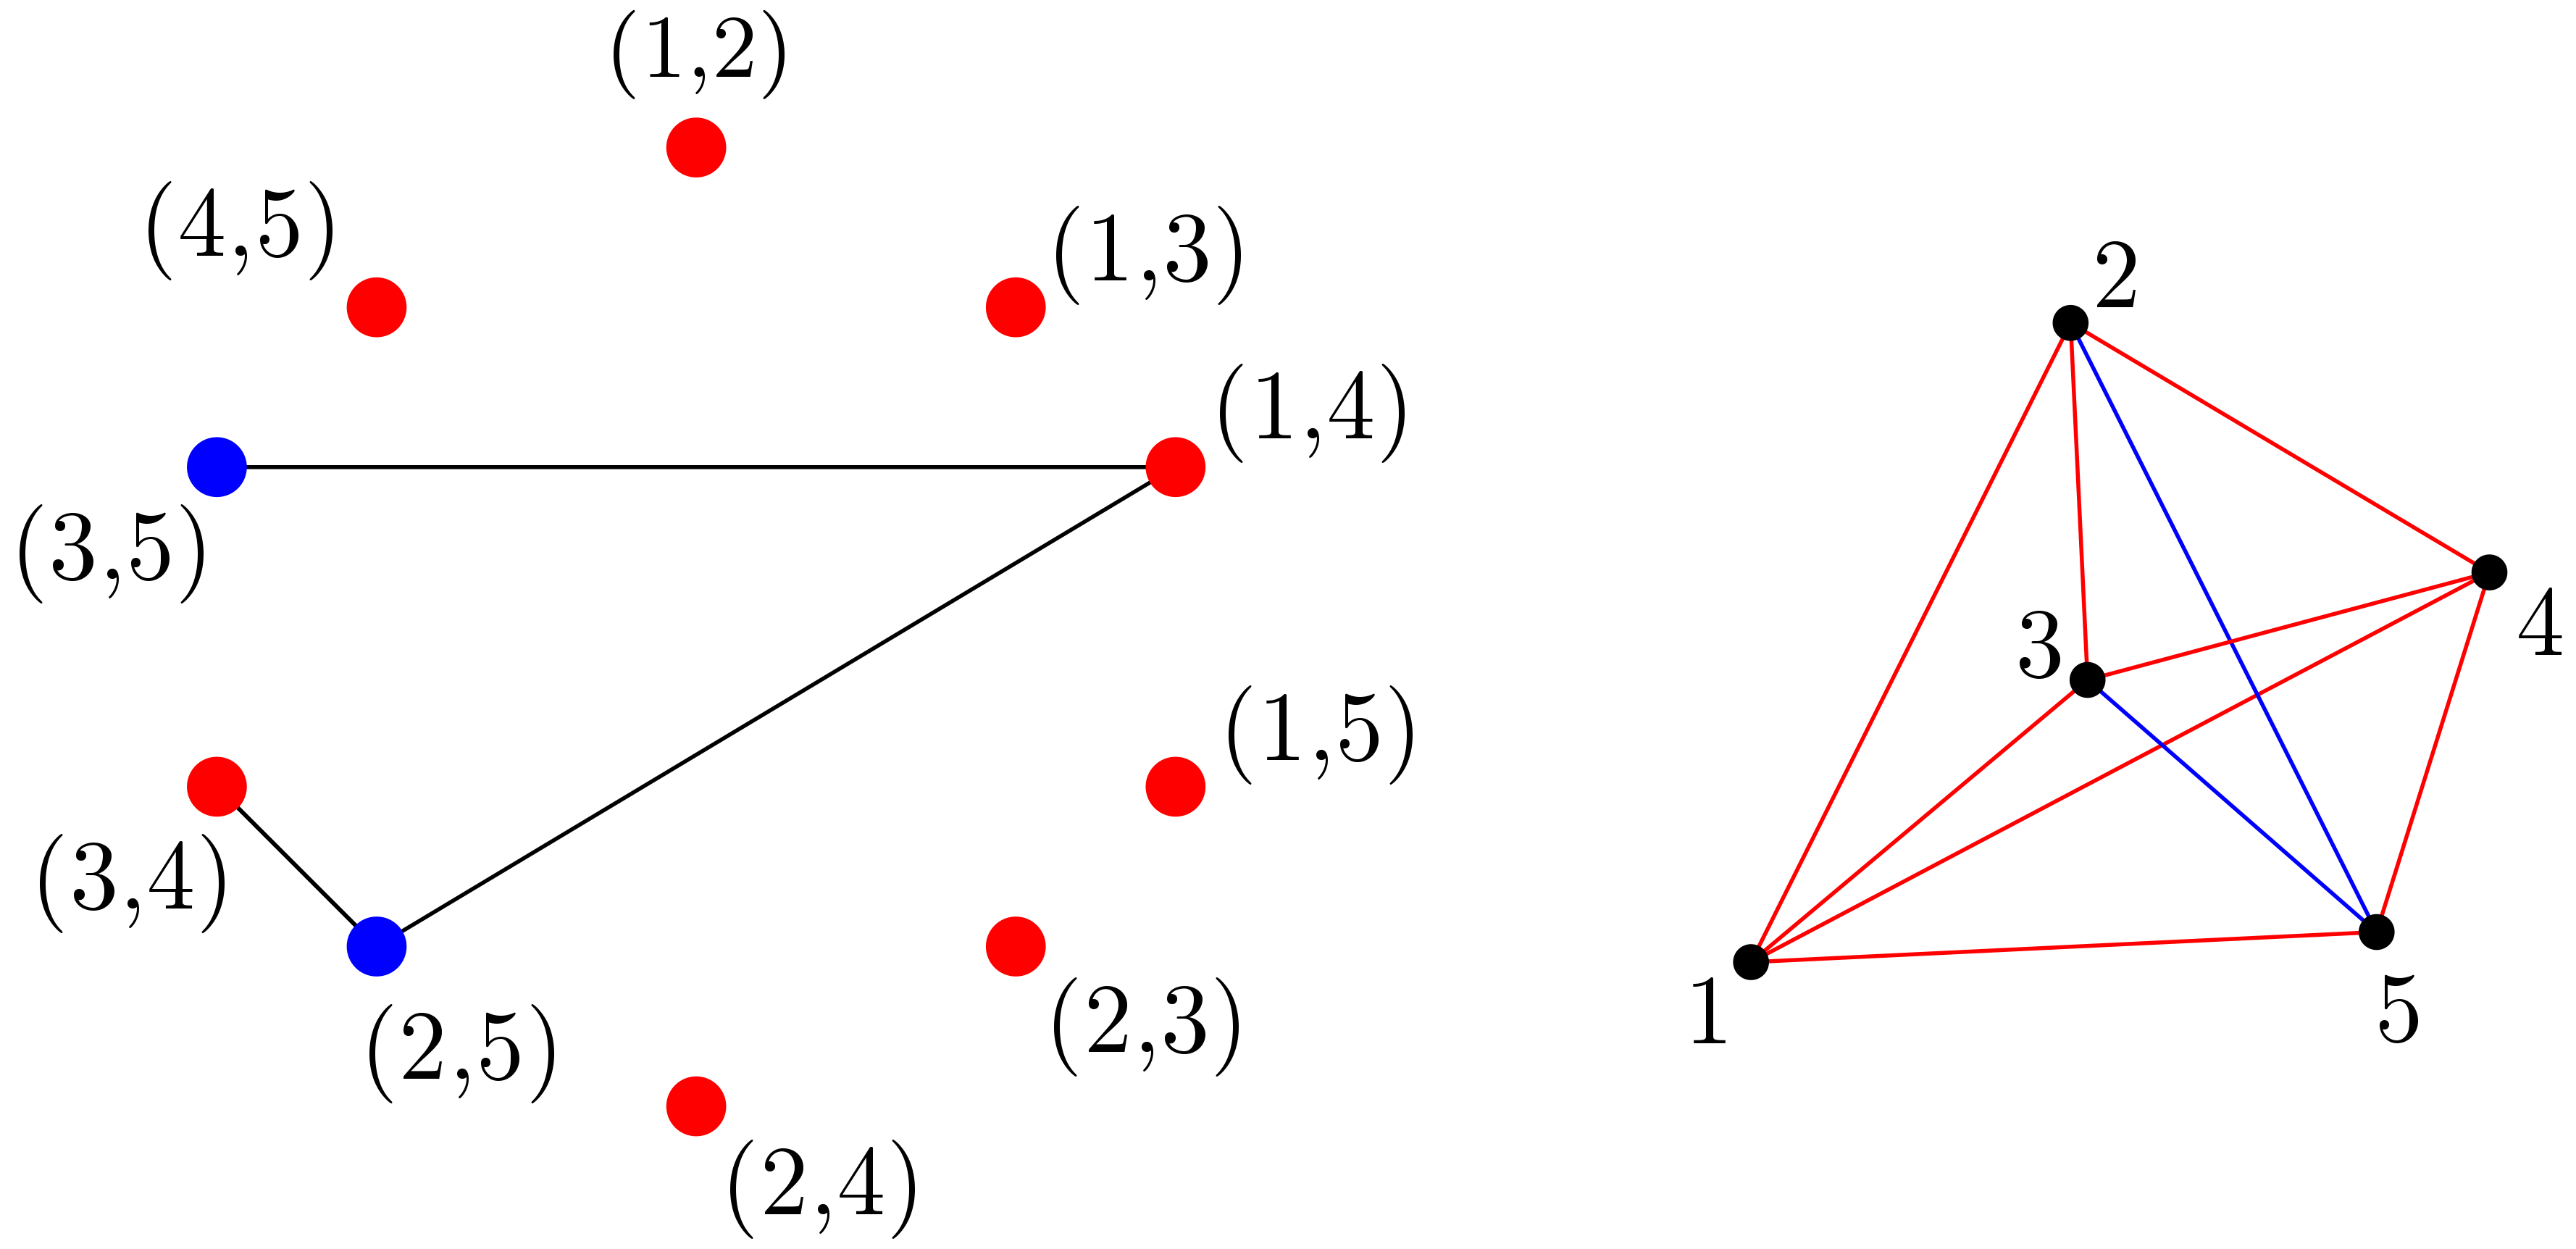
\includegraphics[width=.8\linewidth]{k5coloring}
  \caption{De izquierda a derecha: Una coloración propia de $E_{pp}(S)$ con dos
  clases cromáticas; Una descomposición de un dibujo de $K_5$ en dos gráficas planas
  cuyas aristas corresponden a cada una de las clases cromáticas de la coloración
  de $E_{pp}(S)$.}
  \label{fig:k5coloring}
\end{figure}

De esta manera encontrar el número cromático de la gráfica $E_{pp}(S)$ implica
encontrar el thickness geométrico de $K_n$. Lo que nos permite replantear el thickness
geométrico de un dibujo de la siguiente manera:
\begin{definition}{\emph{Thickness geométrico de un dibujo de una gráfica}.}
  El thickness geométrico $th_g(G)$ de un dibujo geométrico de $G$ es el número cromático
  $\chi(E_{pp}(S))$ de la gráfica $E_{pp}(S)$ donde $S$ es el conjunto de vértices de $K_n$.
\end{definition}
Y luego, siguiendo la definición de \cite{Dillencourt2004} redefinimos el thickness
geométrico de una gráfica completa de $n$ vértices como el thickness geométrico
más pequeño de de todos los dibujos posibles de la gráfica.
A este número le llamaremos también $epp(n)$ y lo definimos formalmente como:
\begin{definition}{\emph{Thickness geométrico de una gráfica}.}
  Considerese $K_n=(S,E)$ la gráfica completa cuyo conjunto de vértices es $S$.
  \[epp(n) = \min\{ \chi(E_{pp}(S)): S \subset \mathbb{R}^2 \text{ está en posición general }, |S|=n \}\]
\end{definition}

De la misma manera que definimos la gráfica de cruce $E_{pp}(S)$ podemos definir
otras gráficas si cambiamos la condición bajo la cual existen aristas entre vértices
de $E_{pp}(S)$. En este sentido, en el trabajo de \cite{Araujo2005}, se definen
varias gráficas que se listan en seguida. Para todas existe una gráfica geométrica
completa $K_n$ cuyo conjunto de vértices es $S$.
\begin{itemize}
  \item $W(S)$ la gráfica en la que existe una arista entre sus vértices
  cuando las aristas correspondientes en $K_n$ no se cruzan propiamente.
  \item $I(S)$ es la gráfica en la que existe una arista entre sus vértices
  cuando las aristas correspondientes en $K_n$ se cruzan propiamente o son adyacentes.
  \item $D(S)$ es la gráfica en la que existe una arista entre sus vértices
  cuando las aristas correspondientes en $K_n$ no se cruzan propiamente ni son adyacentes.
\end{itemize}

Es fácil darse cuenta que la condición de existencia de aristas de $W(S)$ es opuesta
o complementaria a la condición establecida en $E_{pp}(S)$ y viceversa. De la misma
forma, las condiciones de $I(S)$ y $D(S)$ son opuestas entre sí.

En el aporte de \cite{Araujo2005} buscan el número cromático de cada una de las
gráficas listadas anteriormente por lo que creemos sensato decir a qué estructuras
geométricas en el dibujo de $K_n$ equivale una clase cromática de cada alternativa.
Para $W(S)$ una clase cromática equivale a un emparejamiento de cruce (\emph{crossing matching}),
para $I(S)$ equivale a un emparejamiento sin cruce (\emph{non-crossing matching})
y para $D(S)$ equivale a un thrackle.

El hecho de que la coloración de $D(S)$ otorgue una descomposición en thrackles es la
principal razón por la cual el trabajo es de importancia para nosotros. Sin embargo,
en \cite{Araujo2005} se busca el máximo número cromático para cada dibujo posible
de $K_n$ para cada una de las tres gráficas listadas anteriormente. Concretamente
ellos definen los siguiente:

  \begin{align*}
    w(n) &= \max\{\chi(W(S)): S\subset \mathbb{R}^2 \text{ está en posición general }, |S|=n\} \\
    i(n) &= \max\{\chi(I(S)): S\subset \mathbb{R}^2 \text{ está en posición general }, |S|=n\} \\
    d(n) &= \max\{\chi(D(S)): S\subset \mathbb{R}^2 \text{ está en posición general }, |S|=n\} \\
  \end{align*}
Para cada uno también definen el caso en el que $S \subset \mathbb{R}^2$ está
en posición convexa como $w_c(n)$, $i_c(n)$ y $d_c(n)$ y demuestran las siguientes cotas:
\begin{itemize}
  \item $w_c(n) = \Theta(n\log n)$.
  \item $c_1n\log n \leq w(n) \leq c_2 n^2 \frac{\log\log n}{\log n}, \text{ para } c_1,c_2 > 0$.
  \item $i_c(n) = n$.
  \item $n \leq i(n) \leq Cn^{3/2} \text{ para } C > 0$.
  \item $2\lfloor \frac{n+1}{3}\rfloor -1 \leq d_c(n) \leq \min\left( n-2, n - \frac{\lfloor{\log n}\rfloor}{2}\right)$.
  \item $5\lfloor \frac{n}{7}\rfloor \leq d(n) \leq \min\left(n-2,n+\frac{1}{2}- \frac{\lfloor{\log \log n}\rfloor}{n}\right)$.
\end{itemize}
Es importante notar que la definición $d(n)$ no es equivalente a la de anti-thickness
ya que en este último se busca el mínimo número de thrackles en una descomposición.
Entonces podemos dar una definición del anti-thickness geométrico basándonos en la gráfica $D(S)$,
considerando que existe una gráfica completa $K_n = (S,E)$, como sigue a continuación:
\begin{definition}{\emph{Anti-thickness geométrico de una gráfica}.}
  \[gat(n) = \min\{\chi(D(S)): S\subset \mathbb{R}^2 \text{ está en posición general }, |S|=n\}\]
\end{definition}

Y de manera análoga definimos el caso en el que los puntos de $S$ están en posición convexa como
anti-thickness convexo.

\begin{definition}{\emph{Anti-thickness convexo de una gráfica}.}
  \[cat(n) = \min\{\chi(D(S)): S\subset \mathbb{R}^2 \text{ está en posición convexa }, |S|=n\}\]
\end{definition}

Por otro lado, debido a que cuando $K_n$ es dibujado en el plano en posición convexa
los dibujos posibles no presentan diferencias combinatorias se tiene que el
anti-thickness convexo de la gráfica completa de $n$ vértices es equivalente a la definición
de $d_c(n)$ de \cite{Araujo2005}, dicho de otra forma:
\[ d_c(n) = cat(n)\]
% Es natural pensar que si una gráfica puede ser descompuesta en sub-gráficas donde
% no existe ningún cruce entre dos aristas, es quizás posible descomponer la
% gráfica en sub-gráficas donde siempre ocurran cruces entre dos aristas, es decir
% en thrackles; este concepto es conocido como el anti-thickness de una gráfica y
% analogo al caso del thickness también existe el anti-thickness geométrico.

% Antes de examinar los resultados del anti-thickness, resulta interesante verificar
% el trabajo de Araujo y Urrutia \cite{Araujo2005}; aquí se define la gráfica de
% disyunción $D(S)$ de un conjunto $S$ de puntos en el plano, donde considerando
% todos los segmentos de recta entre pares de vértices de $S$ como los vértices
% de $D(S)$, existe una arista entre dos vértices si los dos segmentos
% de recta correspondientes se cruzan o comparten un vértice.

% Si asignamos un color a cada vértice de $D(S)$ de tal manera que dos
% vértices adyacentes no compartan color y además minimizamos el número de colores
% usados, obtenemos el número cromático de $\chi(D(S))$. Es fácil ver que una
% clase cromática de $D(S)$ es un conjunto independiente y además un thrackle. Si
% ahora consideramos todos los posibles encajes de $S$ en el plano y para cada uno
% encontramos $\chi(D(S))$, tendremos una lista de enteros que representa el tamaño
% mínimo de la descomposición en thrackles de una gráfica completa cuyos
% vértices están dados por $S$ en el plano. Si de esta lista consideramos ahora
% el valor mínimo encontraremos el anti-thickness para la gráfica completa geométrica de
% $n$ vértices. Sin embargo, en este trabajo se considera el máximo valor de dicha lista;
% definiendo entonces :
% \[ d(n) = \max\{\chi(D(S)): S \subset \mathbf{R}^2 \text{ en posición general }, |S|=n\}\]
%
% De manera concreta, el trabajo presenta cotas para $d(n)$, y $d_c(n)$ que se define
% de manera similar pero con $S$ en posición convexa.
%
% La diferencia entre $d(n)$ y el anti-thickness reside en que el último buscamos el
% mínimo de la lista de números cromáticos de $D(S)$, para ver más claramente
% la relación entre $d(n)$ y el anti-thickness podemos definir el
% anti-thickness geométrico de la gráfica completa de n vértices $at(n)$ como sigue :
% \[ at(n) = \min\{\chi(D(S)): S \subset \mathbf{R}^2 \text{ en posición general }, |S|=n\}\]

%
% Como se mencionó anteriormente el anti-thickness está relacionado con la descomposición
% de una gráfica en sub-gráficas donde siempre ocurren cruces, podemos ver el
% anti-thickness como el lado opuesto del thickness.
Los autores de \cite{Dujmovic2017} presentan resultados
del anti-thickness para familias específicas de gráficas, por ejemplo árboles, 2-tracks, books, gráficas
outerplanar, k-queues, entre otros haciendo observaciones de resultados anteriores.
Además se prueba la relación entre thickness y anti-thickness, concretamente prueban
la siguiente cota para toda gráfica con anti-thickness $k$ y thickness $t$
: \[ k \leq t \leq \Bigl\lceil \frac{3k}{2}\Bigr\rceil \]

Acerca del anti-thickness (teórico) de gráficas completas, en~\cite{Dujmovic2017}
se prueba que es al menos $\frac{n}{3}$ y a lo más $\lceil \frac{n-1}{2} \rceil$.
Sin embargo ellos conjeturan que el anti-thickness de una gráfica completa es
exactamente $\lceil \frac{n-1}{2} \rceil$.
% Los resultados presentados en ese trabajo que tienen que ver con el anti-thickness
% geométrico de una gráfica completa se enfocan  en el caso específico de puntos en posición convexa.


El principal resultado para posición convexa es presentado en \cite{Fabila-Monroy2018}.
Aquí se prueba que cuando los puntos están en posición convexa dos thrackles máximos
comparten al menos una arista y por lo tanto la unión de $k$ thrackles máximos tiene
a lo más $kn - \binom{k}{2}$ aristas. Luego, como una gráfica completa de $n$
vértices tiene $\binom{n}{2}$ aristas la resolución de la desigualdad
\[ \binom{n}{2} \leq kn - \binom{k}{2} \]
otorga el resultado de la cota inferior para el anti-thickness geométrico convexo que es
\[ n - \Bigl\lfloor \sqrt{2n + \frac{1}{4}} - \frac{1}{2} \Bigr\rfloor \]

La cota superior se obtiene dando una coloración propia de los vértices de la gráfica
de disyunción $D(S)$. La coloración es lograda consiguiendo trazar caminos en una
estructura conocida como polyomino en la que los vértices de $D(S)$ son las filas
y las columnas de dicha estructura. En este trabajo cada camino representa un
conjunto independiente de vértices en $D(S)$ y por lo tanto un thrackle. Concluyen
dando el número máximo de caminos posibles en el polyomino, dicho número coincide con
el de la cota inferior y luego se tiene que el anti-thickness geométrico convexo ($cat(n)$) es:
\[ n - \Bigl\lfloor \sqrt{2n + \frac{1}{4}} - \frac{1}{2} \Bigr\rfloor \]

Es importante notar que el anti-thickness geométrico convexo es acotado examinando el número mínimo
y máximo de aristas aportadas por una colección de thrackles máximos, dicho de
otra manera se basa en descomponer la gráfica completa convexa en thrackles máximos.
Esta idea fue retomada en este trabajo para intentar ajustar las cotas del anti-thickness
en posición general.

Con respecto a puntos que no están estrictamente en posición convexa Leaños y Lomelí~\cite{Lomeli2018}
examinan el número cromático de la gráfica de disyunción de una familia de puntos
conocida como la doble cadena convexa; al igual que la posición convexa la doble cadena
solamente tiene un dibujo en el plano. El resultado al que se llega en este artículo es que
el anti-thickness de la doble cadena convexa con $k$ puntos en la cadena convexa superior
y $l \geq k$ puntos en la cadea convexa inferior es:
 \[k+l-\Bigl\lfloor \sqrt{2l+\frac{1}{4}} - \frac{1}{2} \Bigr\rfloor\]

 Como es mencionado en~\cite{Dujmovic2017}, encontrar el anti-thickness de gráficas
 completas en posición general es un problema abierto y la mejor cota superior
 conocida es $ n - \lfloor \sqrt{2n + \frac{1}{4}} - \frac{1}{2} \rfloor $
la cual se sigue del caso convexo y la mejor cota inferior conocida es solamente
$\lfloor\frac{n-1}{2}\rfloor$ que se sigue del hecho de que una gráfica de $n$ vértices
con anti-thickness geométrico $k$ tiene a lo más $kn$ aristas.
